
\documentclass[timesfont]{MITPress-diacriTech-7x9}


%\usepackage{epsfig}
\usepackage{amsthm}
\usepackage{amssymb}
\usepackage{url}
\usepackage{amsmath}
\usepackage{graphicx}

\input{xypic}

\begin{document}

\frontmatter

\halftitle{Usable Program Security Analysis}


\begin{seriespage}

\seriestitle{Series Title}

\serieseditor{Series Editor}

\begin{seriesentry}
\item Series entry title
\seriesauthor{Author 1}

\item Series entry title
\seriesauthor{Author 2}

\end{seriesentry}

\end{seriespage}

\booktitle{Usable Program Security Analysis}

\subtitle{Subtitle}


\edition{First Edition}

\edauthor{Marco Pistoia\\
	Omer Tripp
}


\MITimprint{The MIT Press\\
Cambridge, Massachusetts\\
London, England}

\begin{copyrightpage}
$\copyright$ 2009 Massachusetts Institute of Technology\\

All rights reserved. No part of this book may be reproduced in any form or by any electronic or mechanical means
(including photocopying, recording, or information storage and retrieval) without permission in writing from the
publisher.\\

For information about special quantity discounts, please email special sales@mitpress.mit.edu.\\

This book was set in Times Roman and Mathtime Pro 2 by the authors.\\

Printed and bound in the United States of America.\\

Library of Congress Cataloging-in-Publication Data\\

Introduction to algorithms / Thomas H. Cormen $\ldots$ [et al.].�3rd ed.\\
\cindent p. cm.\\

Includes bibliographical references and index.\\
ISBN 978-0-262-03384-8 (hardcover : alk. paper)�ISBN 978-0-262-53305-8 (pbk. : alk. paper)\\
1. Computer programming. 2. Computer algorithms. I. Cormen, Thomas H.\\

QA76.6.I5858 2009\\
005.1�dc22\\

\hspace*{12pc}2009008593\\

10\ 9\ 8\ 7\ 6\ 5\ 4\ 3


\end{copyrightpage}


\dedication{Dedication text}

\begin{epigraphpage}
Some text...\source{Source}
\end{epigraphpage}

\tableofcontents

\listoffigures

\listoftables


\begin{contributors}

\name{Thomas H. Cormen}
\affil{Professor and Chair, Department of Computer Science,  Massachusetts Institute of Technology}

\name{Ronald L. Rivest}
\affil{CSAIL, 32 Vassar Street, Room 32-G692, Cambridge MA 02139}


\end{contributors}


\mainmatter

\part{Security: Risks, Threats and Mitigation}

\chapter{Introduction}

\chapter{Foundational Security Principles}

\chapter{Web Security}

\section{OWASP Top Ten for Web}

\section{Cross-site Scripting (XSS)}

\section{SQL Injection (SQLi)}

\chapter{Mobile Security}

\section{OWASP Top Ten for Mobile}

\section{Malware Threats}

\section{Privacy Threats}

\chapter{Other Threats}

\section{Low-level Defects}

\section{Encryption Schemes}

\section{Architectural Defects}

\part{Program Analysis: Background and Foundations}

\chapter{Formal Background}

\section{Graph and Lattice Theory}

\section{Abstract Interpretation}

\section{SAT/SMT Solvers}

\chapter{Intraprocedural Analysis}

\section{Intraprocedural Representations}

\subsection{Control-flow Graph}

\subsection{Static Single Assignment (SSA)}

\section{Semantic Analysis}

\subsection{Dataflow Analysis}

\subsection{Type Checking}

\chapter{Interprocedural Analysis}

\section{Call Graph and Points-to Graph}

\subsection{The Functional Approach}

\subsection{The Call-string Approach}

\section{Whole-program Dataflow Analysis}

\subsection{The Interprocedural Cotrol-flow Graph}

\subsection{IFDS and IDE}

\part{Information-flow Security}

\chapter{Noninterference, Integrity and Confidentiality}

\section{The Principle of Noninterference}

\section{Integrity Threats}

\section{Confidentiality Threats}

\section{Challenges and Limitations}

\chapter{Language-based Approaches}

\section{Implicit Flows}

\section{Compiler Integration}

\section{Challenges and Limitations}

\chapter{Approaches based on Abstract Interpretation}

\section{Taint Analysis}

\section{String Analysis}

\section{Staged Analysis}

\chapter{Other Tools and Techniques}

\section{Hybrid Analysis}

\section{Quantitative and Unit-based Analyses}

\section{Interactive Analyses}

\section{Techniques based on Statistical Learning}

\part{Access Control}

\chapter{Stack-inspection Systems}

\section{Privileged Code}

\section{Support for Multithreaded Programs}

\section{Subjects}

\chapter{Access-rights Analysis}

\chapter{Role-based Access Control: Systems and Analyses}

%\part{Access Control}
%\chapter{Stack-Based Access Control Systems} \label{chap:SBACSystems}

Several modern software platforms---most notably, Java, Standard Edition (SE)
\cite{book:J2SESecBook,book:LiGong}, Java, Enterprise Edition (EE) \cite{book:J2EESecBook} and
Microsoft .NET Common Language Runtime (CLR) \cite{book:DotNetSecurity}---come with an embedded
mechanism for access-control enforcement known as \emph{stack inspection}. 
This chapter describes how Stack-Based Access Control (SBAC)
works.  As a reference, it focuses on the Java SBAC system, which applies
to both Java, SE and Java, EE.  Whenever
necessary, the major differences between the Java and the CLR
SBAC systems will be highlighted.

\section{Basic Concepts}

The Java
and CLR programming models are
extensively used in different kinds of Internet applications,
especially banking, retail and electronic commerce. Due to the
distributed nature of such applications, it is essential that,
when access to a restricted resource is attempted, all code
currently on the call stack is authorized to access that resource.
In Java, the
\texttt{SecurityManager}, if active, triggers access-control
enforcement by invoking \texttt{AccessController.checkPermission}.
This method takes a \texttt{Permission} object \texttt{p} as a
parameter and performs a stack walk to verify that each caller in
the current thread of execution has been granted the access right
represented by \texttt{p}. In CLR, the stack walk is performed by
the \texttt{Demand} method, which verifies that all the code
currently on the stack has been granted the access right
represented by a given \texttt{IPermission} object.

A comparison
between the Java and CLR SBAC systems is shown in Figure
\ref{fig:JVMandCLR}.  The two directed graphs in Figure
\ref{fig:JVMandCLR} represent the executions of two program
threads on a Java and CLR platform, respectively. The vertices
in the graphs represent method invocations.  If two vertices are
connected by an edge, then the method represented by
the predecessor vertex in the edge invokes the method represented
by the successor vertex.  In both platforms, when SBAC is
enforced, a \texttt{SecurityException} is thrown if any one of the
callers on the call stack does not have the appropriate access
right.
\begin{figure}[ht]
	\centering
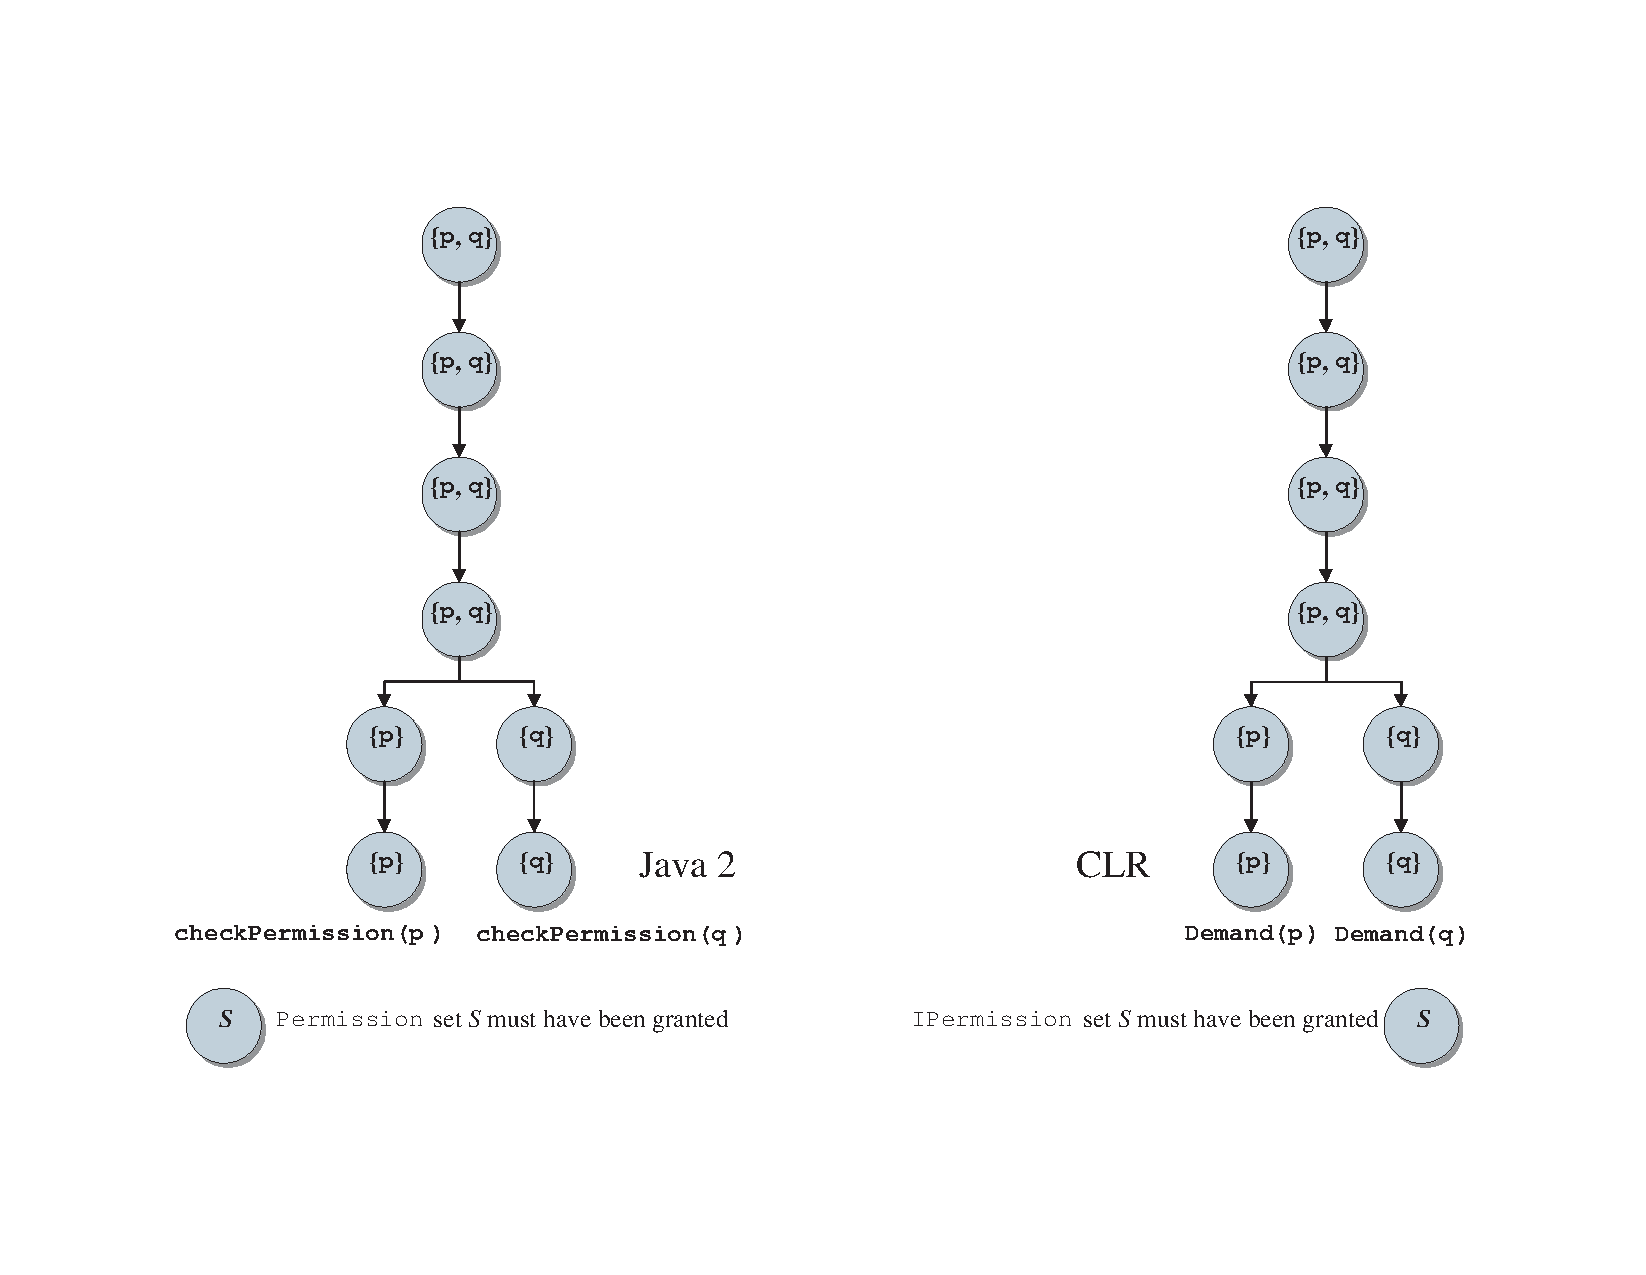
\includegraphics[scale=0.4]{JVMandCLR-eps-converted-to.pdf}
	\caption{The Java and CLR SBAC Systems}
	\label{fig:JVMandCLR}
\end{figure}

\section{Access Rights} \label{sec:AccessRights}

Though programmatic security is possible, in both the Java and
CLR platforms access rights are preferably granted declaratively.
A system administrator grants access rights in a security policy
database that is external to the application code. This enhances
code portability and reusability.  Typically, in SBAC systems,
access rights are by default denied to all code and subjects.
Untrusted code and subjects will only be allowed to perform basic
operations that cannot harm the system.  For a restricted
operation to succeed, all the code on the thread's stack must be
explicitly granted the right to execute that operation.

In Java, access rights are represented as objects of type
\texttt{Permission}. Each \texttt{Permission} type must be a
subclass of the \texttt{Permission} abstract class.  When a
\texttt{Permission} object is constructed, it can take zero, one,
or two \texttt{String} objects as parameters.  If present, the
first parameter is called the \emph{target} of the
\texttt{Permission} object and represents the resource being
protected, whereas the second parameter is called the
\emph{action} of the \texttt{Permission} object and represents the
mode of access. The target and action are used to better qualify
the resource being protected by the \texttt{Permission} object.
For example, the following line of code can be used to construct a
\texttt{Permission} object representing the right to access the
\texttt{log.txt} file in read and write mode:

\begin{tabbing}
	\texttt{Permission p =}\\
	\texttt{   new FilePermission("log.txt",
		"read,write");}
\end{tabbing}

Given a \texttt{Permission} object \texttt{p}, \texttt{p}'s
fully-qualified \texttt{Permission} class name along with
\texttt{p}'s target and action, if any, uniquely identify the
authorization requirement represented by \texttt{p}. Therefore,
for authorization purposes, a \texttt{Permission} object \texttt{p}
can be characterized solely based on its \textit{permission
	ID}, which consists of \texttt{p}'s fully-qualified class name and
the values of the \texttt{String} instances used to instantiate
\texttt{p}.  In fact, in the Java Runtime Environment (JRE)
reference implementation, authorizations are granted to programs
and principals by just listing the corresponding permission IDs in
a flat-file policy database, called the \emph{policy file}
\cite{book:J2SESecBook}.

The \texttt{Permission} class contains an abstract method,
\texttt{implies}, which itself takes a \texttt{Permission} object
as a parameter and returns a \texttt{boolean} value, and that
every non-abstract \texttt{Permission} subclass must implement. If
\texttt{p} and \texttt{q} are two \texttt{Permission} objects and
\texttt{p.implies(q)} returns \texttt{true}, then this means that
granting \texttt{p} is implicitly equivalent to having granted
\texttt{q} as well.  For example, \texttt{p} could be the
\texttt{Permission} object constructed above and \texttt{q} could
be the \texttt{Permission} object constructed with the following line of
code:

\begin{tabbing}
	\texttt{Permission q = new FilePermission("log.txt", "read");}
\end{tabbing}

If \texttt{p} is an instance of the \texttt{AllPermission} class,
then \texttt{p.implies(q)} returns \texttt{true} for any
\texttt{Permission} object \texttt{q}.

Access rights may be granted to code based on the \emph{code
	source}, which is a combination of the \emph{code base}---the
network location from which the code is coming---and the digital
certificates of the entities that digitally signed the code
\cite{book:J2SESecBook}. In Java, access rights are granted to
classes.  Each class is loaded at run time by a class loader.
Class loaders are organized as a tree, called the
\emph{class-loading delegation tree} \cite{book:J2EESecBook}. When
it loads a class, a class loader constructs a \emph{protection
	domain} characterizing the origin of the class being loaded, and
associates it with the class itself. A protection domain, which is
represented as an object of type \texttt{ProtectionDomain},
encapsulates the class' code source (represented as a
\texttt{CodeSource} object) and a \texttt{PermissionCollection}
object containing all the \texttt{Permission}s corresponding to
the access rights granted to that code source.  When it is invoked
with a \texttt{Permission} \texttt{p} as a parameter,
\texttt{checkPermission} performs a stack walk and verifies that
each of the \texttt{ProtectionDomain}s in the current thread of
execution contains in its \texttt{PermissionCollection} at least one \texttt{Permission} that implies
\texttt{p}. The set of \texttt{Permission}s effectively granted to
a thread of execution is the intersection of the sets of
\texttt{Permission}s implied by all the \texttt{ProtectionDomain}s
associated with the stack. Access-control enforcement on a CLR
platform is very similar.

From a security point of view, it should be noted that violations
of the Principle of Least Privilege may arise if unnecessary
rights are granted to code.  Conversely, if the rights granted to
code are insufficient to meet the code's security requirements,
run-time authorization failures may occur, which can cause the
application to crash.

\section{Privileged Code} \label{sec:PrivilegedCode}

Often, trusted library code has been programmed to perform
access-restricted operations---such as writing to a log file or
reading from a configuration file---that its untrusted client did
not explicitly request. Since the untrusted client will be on the
call stack when access control is enforced, the operation will not
succeed unless the client code is authorized as well.  To avoid
authorizing the client, which would constitute a violation of the
Principle of Least Privilege \cite{paper:PrincLeastPriv}, the
portion of library code performing the restricted operation can be
made \emph{privileged}.

In Java, a block of library code is made privileged by wrapping
it into a call to \texttt{AccessController.doPrivileged}. This
method takes either a \texttt{PrivilegedAction} or a
\texttt{PrivilegedExceptionAction} parameter, whose \texttt{run}
method contains the portion of code that needs to be made
privileged.  When access control is enforced, the presence of
privileged code on the call stack causes the stack walk to stop at
the stack frame corresponding to the library method calling
\texttt{doPrivileged}. As a result, the library code calling
\texttt{doPrivileged} must have been granted the right to perform
the restricted operation, but the client code is implicitly
granted that right while the current thread is executing.  A
potential problem generated by \texttt{doPrivileged} is that, if a
call to \texttt{doPrivileged} leads to multiple
\texttt{checkPermission} calls with different \texttt{Permission}s
being checked, all those \texttt{Permission}s will be implicitly
granted to client code indiscriminately.

In CLR, the mechanism for privileged code is more granular.  To
make code privileged, a trusted library code must call the
\texttt{Assert} method with an \texttt{IPermission} object
\texttt{p} as a parameter. The difference from Java's
\texttt{doPrivileged} is that \texttt{Assert} does not cause the
stack walk to stop, but instead adds \texttt{p} to the stack
frames above the library method that makes the call to
\texttt{Assert}.  Therefore, unlike \texttt{doPrivileged},
\texttt{Assert} allows specifying exactly which access right
should be implicitly granted to client code, regardless of the
\texttt{IPermission} being checked by the \texttt{Demand} method
currently on the stack.  Figure \ref{fig:privilegedcode} shows and
compares how privileged code works in the Java and CLR
platforms, respectively.

\begin{figure}[ht]
	\centering
	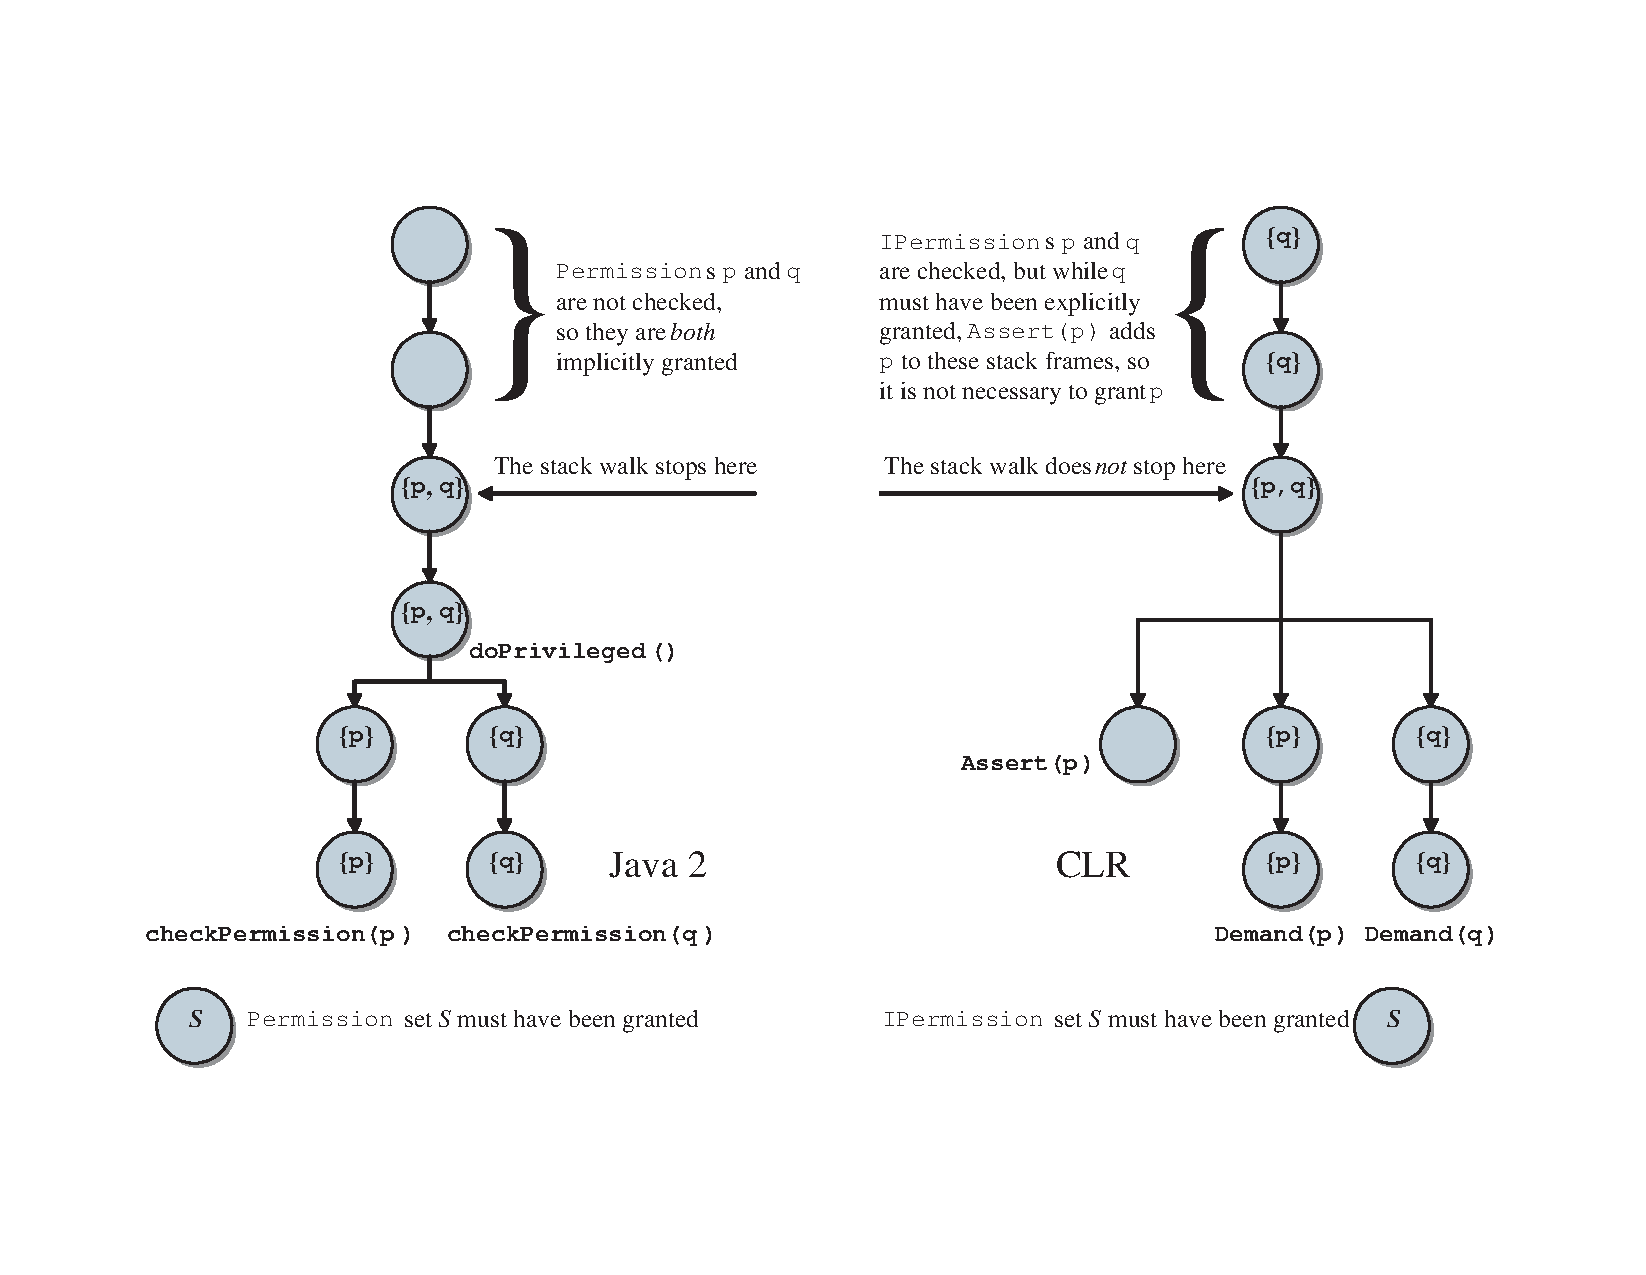
\includegraphics[scale=0.4]{privilegedcode-eps-converted-to.pdf}
	\caption{Privileged Code in the Java and CLR SBAC Systems}
	\label{fig:privilegedcode}
\end{figure}

The Java platform offers another form of \texttt{doPrivileged}
that takes an additional \texttt{AccessControlContext} instance as
an argument.  This instance encapsulates an array of
\texttt{ProtectionDomain} objects, which are typically those
associated with the thread stack at the moment in which the
\texttt{AccessControlContext} was instantiated. When it encounters
a call to this form of \texttt{doPrivileged},
\texttt{checkPermission} stops its stack walk at the stack frame
corresponding to the method that made that \texttt{doPrivileged}
call. However, in addition, \texttt{checkPermission} performs an
authorization test on each of the \texttt{ProtectionDomain}s
encapsulated in the \texttt{AccessControlContext}.

The remainder of this section further describes the problems that
can be introduced with privileged code.

\subsection{Library Code Access Control} \label{sec:LibraryCodeAC}
When a client application makes a call into a trusted library, the
library often accesses restricted resources that the client never
intended to, nor does it need to, directly access. For instance,
assume that a Java program is authorized to open a network socket.
To do so, it invokes \texttt{createSocket} on the
\texttt{LibraryCode} library class in Figure
\ref{fig:LibraryCode1}.
\begin{figure*}[h]
	\begin{tabbing}
		\hspace*{0.25in}\=\hspace*{0.25in}\=\hspace*{0.25in}\=\hspace*{0.25in}\kill
		\texttt{import java.io.*;}\\
		\texttt{import java.net.*;}\\
		\verb"public class LibraryCode {"\\
			\>\texttt{private static String logFileName = "audit.txt";}\\
			\>\verb"public static Socket createSocket(String host, int port)"\\
			\>\>\>\verb"throws UnknownHostException, IOException {"\\
				\>\>\texttt{// Create the Socket}\\
				\>\>\texttt{Socket socket = new Socket(host, port);}\\
				\>\>\texttt{// Log the Socket operation to a file}\\
				\>\>\texttt{FileOutputStream fos = new FileOutputStream(logFileName);}\\
				\>\>\texttt{BufferedOutputStream bos = new BufferedOutputStream(fos);}\\
				\>\>\texttt{PrintStream ps = new PrintStream(bos, true);}\\
				\>\>\texttt{ps.print("Socket " + host + ":" + port);}\\
				\>\>\texttt{return socket;}\\
				\>\verb"}"\\
			\verb"}"
	\end{tabbing}
	\caption{Library Code Propagating Authorization Requirements to
		Its Clients} \label{fig:LibraryCode1}
\end{figure*}

On opening a socket on behalf of a client program, the library is
programmed to log the socket operation to a file for auditing
purposes. As shown in Figure \ref{fig:NoDoPriv}, according to the
Java SBAC model, both the library and its client will need to be
granted the \verb"FilePermission" to modify the log file and the
\verb"SocketPermission" to create the socket connection, even
though the client did not explicitly request to write to the log
file. Granting that \texttt{FilePermission} to the client code
would violate the Principle of Least Privilege.
\begin{figure*}[h]
	\centering
	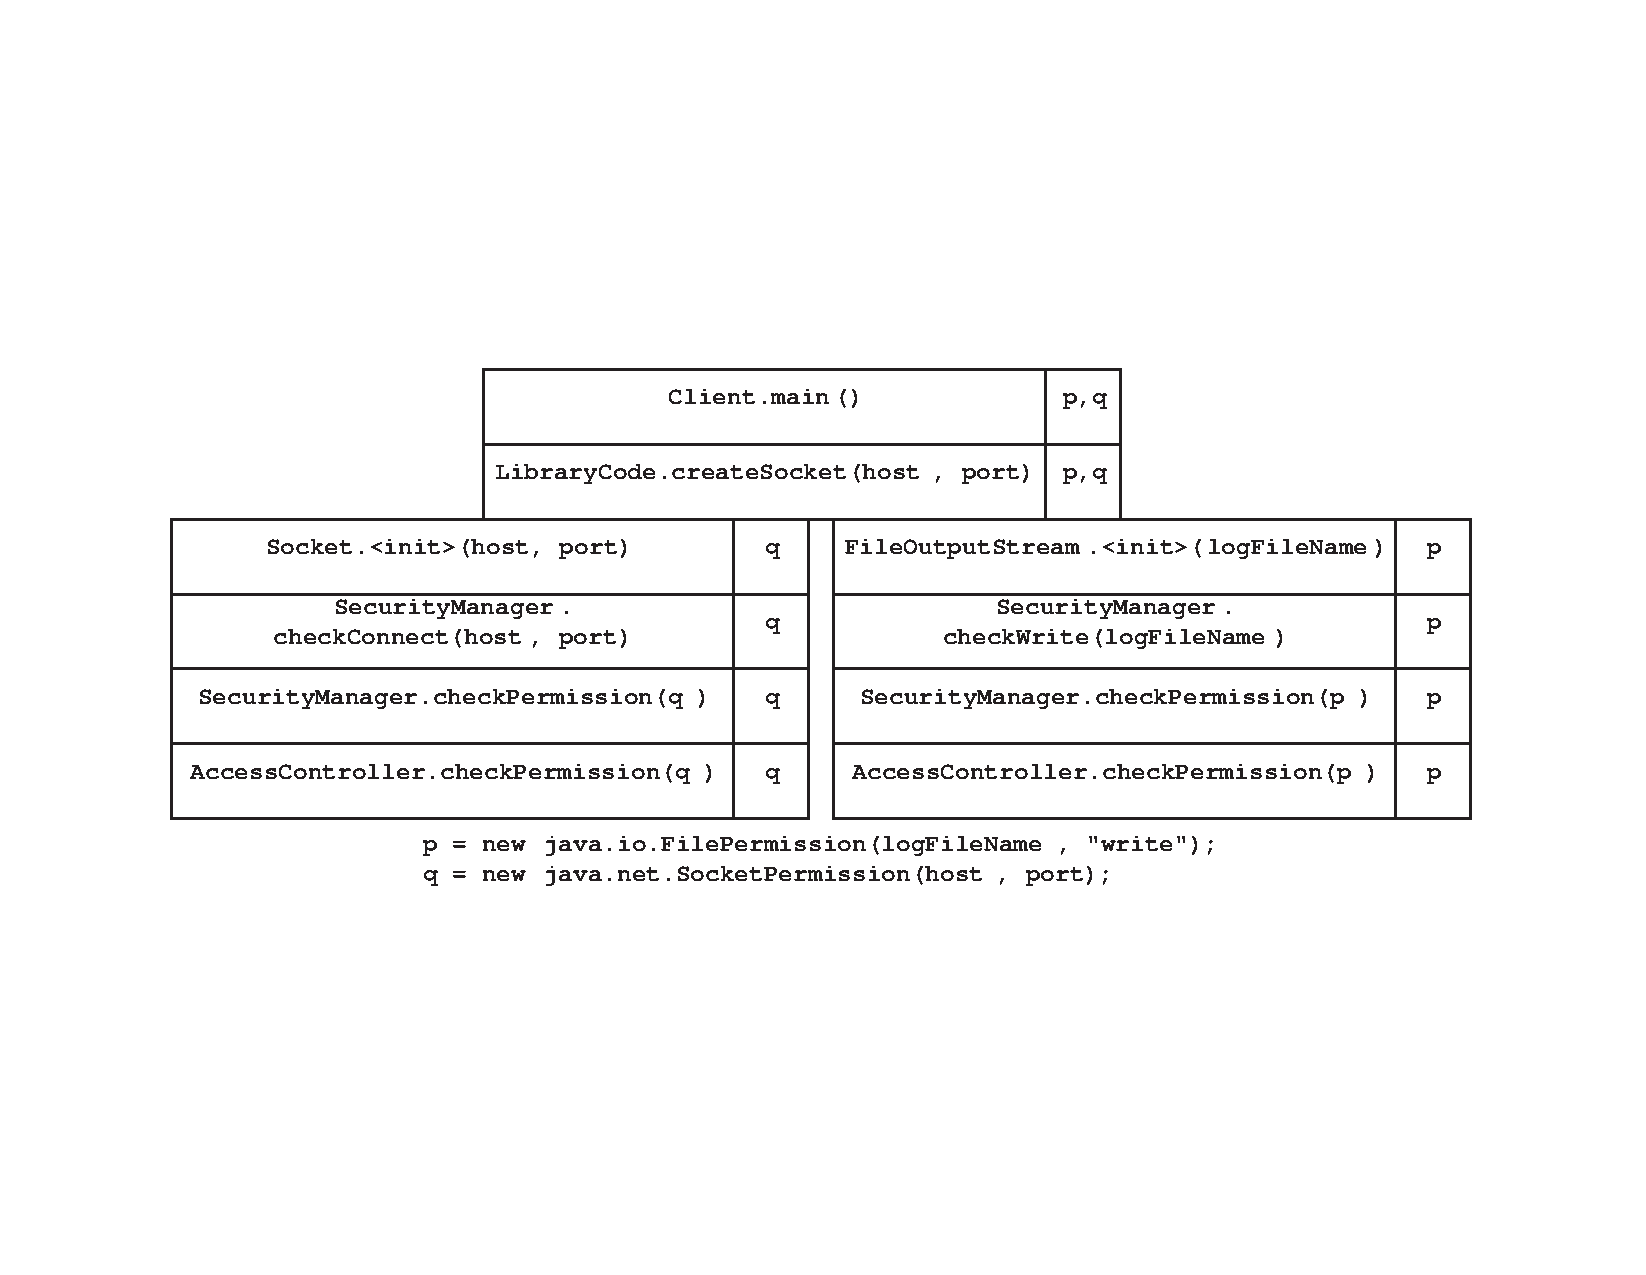
\includegraphics[scale=0.4]{pistoia-figure1-eps-converted-to.pdf}
	\caption{Propagating Unnecessary Authorization Requirements to Client Code}
	\label{fig:NoDoPriv}
\end{figure*}

One way to circumvent this problem is to mark the portion of the
library code responsible for logging as privileged. On a Java
platform, this prevents the stack inspection for the log operation
from going beyond the \texttt{createSocket} method, and
temporarily exempts the client from the \texttt{FilePermission}
requirement during the execution of \texttt{createSocket}. From a
practical point of view, a Java developer must implement either
the \verb"PrivilegedExceptionAction" or \verb"PrivilegedAction"
interface, depending on whether the privileged code could throw a
checked \verb"Exception" or not, respectively.  Both these
interfaces have a \verb"run" method that, once implemented, must
contain the portion of library code performing the restricted
operation not directly requested by the client. Next, the
\verb"PrivilegedExceptionAction" or \verb"PrivilegedAction"
instance is passed as a parameter to the \verb"doPrivileged"
method, which will invoke the instance's \texttt{run} method.

\begin{figure*}
	\begin{tabbing}
		\hspace*{0.25in}\=\hspace*{0.25in}\=\hspace*{0.25in}\=\hspace*{0.25in}\=\hspace*{0.25in}\kill
		\verb"import java.io.*;"\\
		\verb"import java.net.*;"\\
		\verb"import java.security.*;"\\
		\verb"public class LibraryCode2 {"\\
			\>\texttt{private static final String logFileName = "audit.txt";}\\
			\>\texttt{public static Socket createSocket(String host, int port) throws}\\
			\>\>\>\verb"UnknownHostException, IOException, PrivilegedActionException {"\\
				\>\>\texttt{// Create the Socket}\\
				\>\>\texttt{Socket socket = new Socket(host, port);}\\
				\>\>\texttt{// Log the Socket operation to a file using doPrivileged}\\
				\>\>\texttt{File f = new File(logFileName);}\\
				\>\>\texttt{PrivWriteOp op = new PrivWriteOp(host, port, f);}\\
				\>\>\texttt{FileOutputStream fos = (FileOutputStream)}\\
				\>\>\>\>\texttt{AccessController.doPrivileged(op);}\\
				\>\>\texttt{BufferedOutputStream bos = new
					BufferedOutputStream(fos);}\\
				\>\>\texttt{PrintStream ps = new PrintStream(bos, true);}\\
				\>\>\texttt{ps.print("Socket " + host + ":" + port);}\\
				\>\>\texttt{return socket;}\\
				\>\verb"}"\\
			\verb"}"\\
		\verb"class PrivWriteOp implements PrivilegedExceptionAction {"\\
			\>\texttt{private File f;}\\
			\>\verb"PrivWriteOp (File f) {"\\
				\>\>\verb"this.f = f;"\\
				\>\verb"}"\\
			\>\verb"public Object run() throws IOException {"\\
				\>\>\texttt{return new FileOutputStream(f);}\\
				\>\verb"}"\\
			\verb"}"
	\end{tabbing}
	\caption{Library Using Privileged Code} \label{fig:LibraryCode2}
\end{figure*}

Class \texttt{LibraryCode2} in Figure \ref{fig:LibraryCode2} is
obtained by modifying class \verb"LibraryCode" in Figure
\ref{fig:LibraryCode1}. The main modification consists of wrapping
the call to the \texttt{FileOutputStream} constructor in a
privileged block to prevent client code from requiring a
\verb"FilePermission".

\begin{figure*}[h]
	\centering
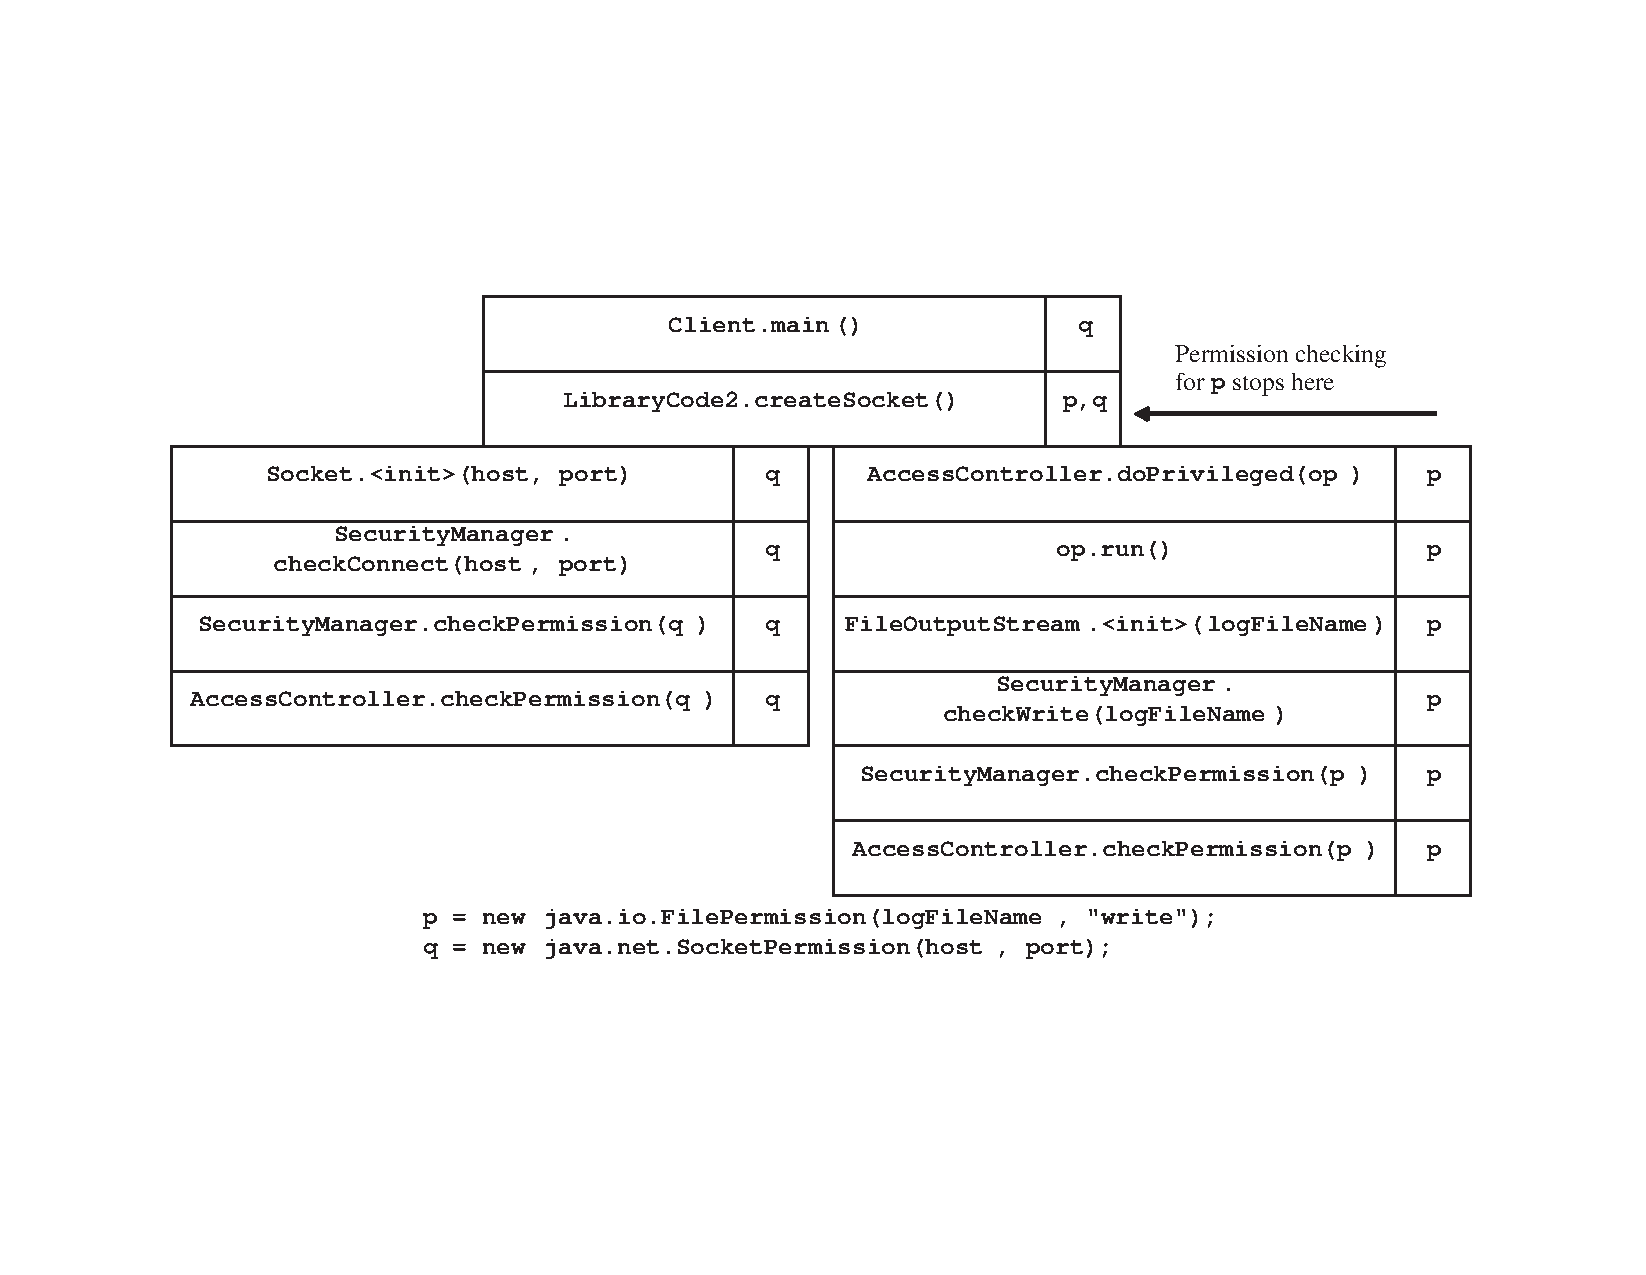
\includegraphics[scale=0.4]{pistoia-figure2-eps-converted-to.pdf}
	\caption{Preventing Unnecessary Authorization Requirements for Client Code}
	\label{fig:withDoPriv}
\end{figure*}

As shown in Figure \ref{fig:withDoPriv}, when the
\verb"checkPermission" method performs a stack walk to verify that
all the code in the active calling sequence has been granted the
right to write to the log file, the \verb"LibraryCode2" class will
be required to have the necessary \verb"FilePermission", but the
client code running on top of it will not.  However, the client
code will still be required to have the \verb"SocketPermission"
necessary to open the socket since the call to the \verb"Socket"
constructor in \verb"LibraryCode" is not privileged.

\subsection{Correct Placement of Privileged Code}
Taking preexisting library code and understanding which portions
of it should be made privileged by performing manual code
inspection is a difficult task, which is even more challenging
when the library is large or complex. Besides identifying the
blocks of library code that require authorizations, developers
must understand which authorizations are implicitly granted to
possibly unknown client code when the library code is made
privileged.

Frequently, libraries are not written with security as a concern,
or they are written to run on a version of the Java Runtime
Environment (JRE) prior to 1.2.\footnote{The Java fine-grained
	access control model was introduced in version 1.2.} When a Java
\texttt{SecurityManager} is finally turned on for a particular
application, \texttt{SecurityException}s are thrown due to access
control violations. It may be very difficult to understand which
portions of library code should be made privileged in order to
prevent client code from requiring unnecessary authorizations that
are only needed by the library code.

In practice, this problem is solved empirically. The developer
tests the library code with sample client code that makes calls
into the library. Typically, the client code is granted only a
limited number of authorizations, while the library is granted
sufficient authorizations, such as \verb"AllPermission". Next, it
is necessary to take note of all the \verb"SecurityException"s
generated when running the test cases, and to distinguish between
two categories of \verb"SecurityException"s:
\begin{enumerate}
	\item The \verb"SecurityException"s due to the client code's attempting to
	access some restricted resources through the library without
	the adequate authorizations
	\label{list:SecurityExceptionsOfType1}
	\item The \verb"SecurityException"s due to the library's attempting
	to access some restricted resources on its own without using
	privileged code \label{list:SecurityExceptionsOfType2}
\end{enumerate}
Eliminating a \verb"SecurityException" of category
\ref{list:SecurityExceptionsOfType2} requires inspecting the
library source code, identifying which portion of it is
responsible for accessing the protected resource, and making that
portion of code privileged. A \verb"SecurityException" of category
\ref{list:SecurityExceptionsOfType1} can instead be eliminated by
granting the client code the necessary access rights, but this
operation must be performed cautiously because granting
authorizations to the client could hide \verb"SecurityException"s
of category \ref{list:SecurityExceptionsOfType2}. Manually
performing this task is difficult, tedious, and error-prone. After
modifying the library code or the client security policy, the
developer must rerun the test cases. This process must be
repeated, possibly many times, until there are no more
authorization failures. Additionally, \verb"doPrivileged"
requirements in the library code may remain undiscovered during
testing due to an insufficient number of test cases, which makes
production code potentially unstable.

It is also important to avoid introducing ``unnecessary'' and
``redundant'' privileged blocks code.  Privileged code is
\emph{unnecessary} if there is no path from it to any security
check, and it is \emph{redundant} if all the security checks it
leads to are covered by other privileged code. Unnecessary or
redundant privileged code may lead to violations of the Principle
of Least Privilege, especially during subsequent code maintenance.
Additionally, from a performance point of view, it can be
expensive.  Therefore, such code should be made unprivileged.

\subsection{Tainted Variables}

A variable in a program is said to be \emph{tainted} if its value
can be arbitrarily set by the client code
\cite{Web:SecCodeGuidelines}. For example, if the privileged code
is responsible for writing to a log file, the name of the log file
should not be a tainted variable, or an untrusted caller could
invoke that privileged code and modify any file in the file
system.

A tainted variable is not necessarily a security problem.  In Java
2, a tainted variable may constitute a security problem if it is
also a \emph{privileged} variable, meaning that it is used inside
privileged code \cite{Web:SecCodeGuidelines}.  Even a tainted
privileged variable is not necessarily a security problem.  In
fact, it is possible to distinguish two types of privileged
tainted variables: if a privileged tainted variable is used to
access a restricted resource, it is said to be \emph{malicious},
otherwise it is said to be \emph{benign}. Since security checks
are not performed beyond the stack frame invoking
\texttt{doPrivileged}, an untrusted client application could
exploit a malicious variable to have the privileged code access
restricted resources on its behalf. Consider, for example, the
\texttt{GetSocket} utility class shown in Figure
\ref{fig:helperMethod}. Both \texttt{host} and \texttt{port} are
tainted variables, since an untrusted client can arbitrarily set
them. The fact that they are used inside privileged code to open a
socket makes them malicious and constitutes a potential security
risk.  An untrusted client, with no \texttt{SocketPermission}, can
invoke \texttt{getSocket} on the trusted library and have the
library open an arbitrary socket connection on its behalf.
Conversely, variable \texttt{userName}, though tainted and
privileged, is benign since its value is not used to access a
restricted resource.  In Figure \ref{fig:LibraryCode2}, variable
\texttt{logFileName} is not tainted because its value cannot be
set by a client application.

\begin{figure*}
	\begin{tabbing}
		\hspace*{0.25in}\=\hspace*{0.25in}\=\hspace*{0.25in}\=\hspace*{0.25in}\=\hspace*{0.25in}\=\hspace*{0.25in}\kill
		\texttt{import java.net.*;}\\
		\texttt{import java.security.*;}\\
		\verb"public class GetSocket {"\\
			\>\verb"public static Socket getSocket(final String host, final int port,"\\
			\>\>\>\verb"final String userName) throws Exception {"\\
				\>\>\texttt{Socket s;}\\
				\>\>\texttt{PrivOp op = new PrivOp(host, port, userName);}\\
				\>\>\verb"try {"\\
					\>\>\>\texttt{s = (Socket) AccessController.doPrivileged(op);}\\
					\>\>\verb"}"\\
				\>\>\verb"catch (PrivilegedActionException e) {"\\
					\>\>\>\verb"throw e.getException();"\\
					\>\>\verb"}"\\
				\>\>\texttt{return s;}\\
				\>\verb"}"\\
			\verb"}"\\
		\verb"class PrivOp implements PrivilegedExceptionAction {"\\
			\>\texttt{private String host, userName;}\\
			\>\texttt{int port;}\\
			\>\verb"PrivOp(String host, int port, String userName) {"\\
				\>\>\verb"this.host = host;"\\
				\>\>\verb"this.port = port;"\\
				\>\>\verb"this.userName = userName;"\\
				\>\verb"}"\\
			\>\verb"public Object run() throws Exception {"\\
				\>\>\texttt{System.out.println("Received request from user " + userName);}\\
				\>\>\verb"return new Socket(host, port);"\\
				\>\verb"}"\\
			\verb"}"
	\end{tabbing}
	\caption{Helper \texttt{getSocket} Method with Tainted Parameters}
	\label{fig:helperMethod}
\end{figure*}

Sometimes, it may be necessary to use tainted variables inside
privileged code to access restricted resources. In such cases it
is important to perform \emph{sanity checks} on those variables to
verify that they satisfy certain preconditions
\cite{paper:AshcraftEngler2002}. For example, in the code of
Figure \ref{fig:helperMethod}, the programmer could
\emph{sanitize} \texttt{host} and \texttt{port} and make them
untainted by refusing to execute the privileged code if, for
example, the \texttt{host} value does not end with \texttt{.edu}
and the \texttt{port} value is different from \texttt{443}.

In general, manually ensuring that no tainted variables are used
inside privileged code to access restricted resources is time
consuming and error prone. It requires:
\begin{enumerate}
	\item Identifying all the unsanitized, malicious tainted
	variables (such as \texttt{host} and \texttt{port} in Figure \ref{fig:helperMethod})
	and separating them from the benign ones (such as \texttt{userName})
	\item Determining all the control- and data-flow paths in the execution of the library that
	would allow an unsanitized, malicious tainted variable to be
	used inside some privileged code to access restricted
	resources
\end{enumerate}

Determining if the code candidate to become privileged uses
unsanitized, malicious tainted variables to access restricted
resources helps when deciding whether making that code privileged
is appropriate or not. For example, the code of Figure
\ref{fig:LibraryCode1} has two instructions that could be made
privileged:
\begin{enumerate}
	\item \texttt{Socket socket = new Socket(host, port);}
	\label{list:socket}
	\item \texttt{FileOutputStream fos = new FileOutputStream(logFileName);}
	\label{list:file}
\end{enumerate}
If Instruction \ref{list:socket} is made privileged, then
parameters \verb"host" and \verb"port", which are tainted, will
constitute a security exposure since they are used to access a
restricted resource. This is an indication that Instruction
\ref{list:socket} should not be made privileged. Conversely,
parameter \verb"logFileName" is not tainted. This is an indication
that Instruction \ref{list:file} could be made privileged.

\section{Multi-Threaded Programs} \label{sec:multi-threadedprograms}
In the Java SBAC system, when
access to a restricted resource is attempted from within a child
thread, it is not just the code on the stack of the child thread
that must be granted the right to perform the access-restricted
operation, but all the code in the child thread and in all its
ancestor threads. This is done to prevent a program from
performing security-sensitive operations by simply spawning a new
thread, which would have fewer classes associated with the
run-time stack, and be therefore potentially more trusted than its
ancestor threads.

\section{Subjects-Based Authorization} \label{sec:SubjectBasedAuthorization}
Both Java and CLR allow basing authorization decisions on the user
or service, called the \emph{subject}, executing the code.  Java
Authentication and Authorization Service (JAAS) extends the Java
code-based access control framework to support subject-based
authentication and authorization
\cite{book:J2EESecBook,paper:jaas}.  In Java, a subject is
represented as an object of type \texttt{Subject}. When a subject
is authenticated, the corresponding \texttt{Subject} instance is
populated with associated identities called \emph{principals},
represented as objects of type \texttt{Principal}. A subject may
have multiple associated principals.  For example, if the subject
is a person, two of the subject's associated principals could be
the person's name and social security number.

In Java, access rights are granted to code and principals, but
not directly to subjects. The set of access rights granted to a
subject is obtained as the union of the sets of access rights
granted to the subject's authenticated principals. The JAAS
framework offers the static methods \texttt{Subject.doAs} and
\texttt{Subject.doAsPrivileged} to perform a restricted operation
with the access rights granted to a subject.

\begin{itemize}
	\item The \texttt{doAs} method takes two parameters: the first
	is a \texttt{Subject} object, and the second is either a \texttt{PrivilegedAction} or
	\texttt{PrivilegedExceptionAction} object.  The code in the
	\texttt{run} method of the \texttt{PrivilegedAction} or
	\texttt{PrivilegedExceptionAction} instance is executed with the
	intersection of the sets of \texttt{Permission}s granted to the
	code on the call stack. However, \texttt{doAs} adds the
	\texttt{Permiossion}s granted to the subject's principals to the
	stack frames subsequent to the call to \texttt{doAs}.
	\item The \texttt{doAsPrivileged} method is similar to
	\texttt{doAs}, but it takes a third parameter, an
	\texttt{AccessControlContext} object, which encapsulates an array
	of \texttt{ProtectionDomain}s. Just like \texttt{doAs}, the \texttt{doAsPrivileged}
	method also adds the \texttt{Permission}s granted to the subject's
	principals to the subsequent stack frames. However, unlike in the \texttt{doAs} case, when
	\texttt{checkPermission} is called with a \texttt{Permission}
	parameter \texttt{p} after a call to \texttt{doAsPrivileged},
	the \texttt{doAsPrivileged} predecessors are not required to
	have been granted a \texttt{Permission} that implies \texttt{p}.
	Rather, \texttt{doAsPrivileged} interrogates the
	\texttt{ProtectionDomain}s in the \texttt{AccessControlContext}
	passed to it as a parameter \cite{book:J2EESecBook}.
\end{itemize}

Violations of the Principle of Least Privilege may arise if any of
the access rights granted to a subject's principals are
unnecessary.  Conversely, if the rights granted are insufficient
to meet the security requirements of an application, run-time
authorization failures may occur, which could cause the
application to crash.

Similar to privileged code, code executed under the authority of a
subject can be ``unnecessary'' or ``redundant.'' Specifically, a
call to \texttt{doAs} or \texttt{doAsPrivileged} is
\emph{unnecessary} if it does not lead to any
\texttt{checkPermission} call, and it is \emph{redundant} if all
the \texttt{checkPermission} calls it leads to are covered by
calls to \texttt{doPrivileged}. Code unnecessarily or redundantly
executed under the authority of a subject may lead to violations
of the Principle of Least Privilege, especially during subsequent
code maintenance. Additionally, from a performance point of view,
it can be expensive.


%
%\chapter{Information-flow Security}


\end{document}
